\section{Experimental Setup}

\subsection*{Circuit components}
    \begin{enumerate}
        \item Inductor
        \item Capacitor
        \item Resistors
        \item Function generator
        \item Oscilloscope
        \item Multimeter/LCR meter
        \item Connecting wires
        \item Breadboard
    \end{enumerate}

    \subsection*{Circuit Diagram}
    Given in Fig. \ref{fig:1}.

\section{Data Analysis and Calculations}

\begin{itemize}
    \item $L=952.4\,\mu$H 
    \item $C=75.41\,$nF
    \item $f_o=\frac{1}{2\pi\sqrt{LC}}=18.78$ kHz
    \item Internal resistance of inductor $= 11.8\,\Omega$
    \item Output impedance of Function generator $= 50\,\Omega$
    \item $R_1=98.4\,\Omega$ and $R_2=46.1\,\Omega$
\end{itemize}

    \subsection{$V_R/V_i$ vs frequency plot}

        \begin{figure}[H]
            \centering
            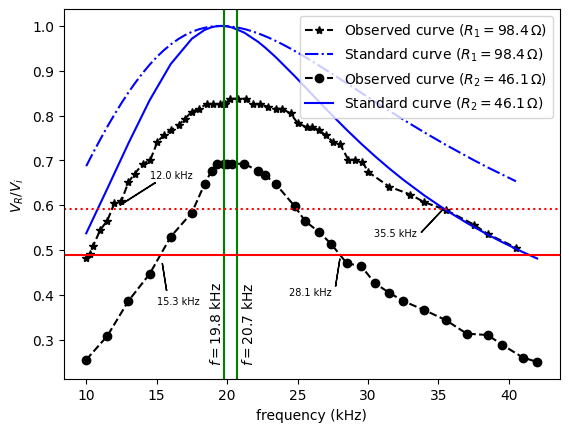
\includegraphics[width=1\columnwidth]{images/g2.png}
            \caption{Observed and computed values of $V_R/V_i$ vs input frequency plotted for two values of resistances}
            \label{graph:1}
        \end{figure}

        From Fig. \ref{graph:1} we can graphically estimate the resonant frequency of the circuit (as when the curve reaches the maxima):

        \begin{itemize}
            \item $f_o$ (when $R_1=98.4\,\Omega$) = 20.7 kHz
            \item $f_o$ (when $R_2=46.1\,\Omega$) = 19.8 kHz
        \end{itemize}

        Hence the average value of resonant frequency would be $f_o=20.05$ kHz.

        Q-factor for both resistances can be calculated using Eqn. (7), 

        \begin{itemize}
            \item $Q_1$ (for $R_1$) = 0.773
            \item $Q_2$ (for $R_2$) = 1.098
        \end{itemize}

        Q-factor can also be estimated from the plot by finding $f_2$ and $f_1$ as the values where $V_R/V_i$ becomes $1/\sqrt{2}=0.707$ of the maximum value.
        
        \begin{itemize}
            \item For $R_1$, these points come out to be $f_1 = 12.0$ kHz and $f_2 = 35.5$ kHz. Hence using Eqn. (8), we can calculate Q factor to be $Q_1=0.881$.
            \item For $R_2$, $f_1 = 15.3$ kHz and $f_2 = 28.1$ kHz. Hence using Eqn. (8), $Q_2=1.547$.
        \end{itemize}

        Here we can see that for both methods, Q-factor of $R_1$ is lower that that of $R_2$, which means resistive energy loss will be higher in the first circuit (with higer $R_{dc}$). Higher Q-factor means better selectivity and thus a narrower bandwidth.

    \subsection{$\phi_R$ vs frequency plot}

        \begin{figure}[H]
            \centering
            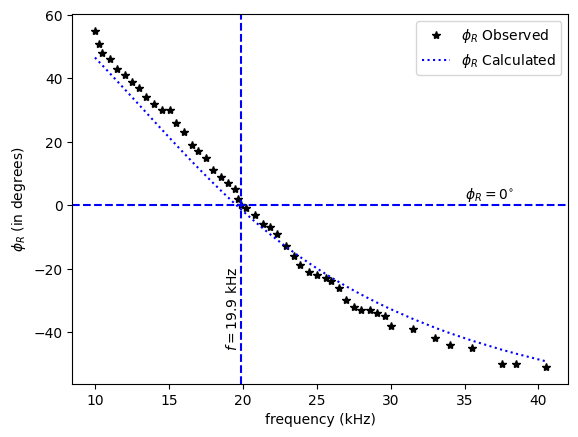
\includegraphics[width=1\columnwidth]{images/g1.png}
            \caption{Observed and computed values of $\phi_R$ vs input frequency plotted for $R_1=98.4\,\Omega$}
            \label{graph:2}
        \end{figure}

        At resonance, $\phi_R=0$ and hence we can est the resonance frequency as $f_o=19.9$ kHz

    \subsection{$V_{LC}/V_i$ and $\phi_{LC}$ vs frequency plots}

        \begin{figure}[H]
            \centering
            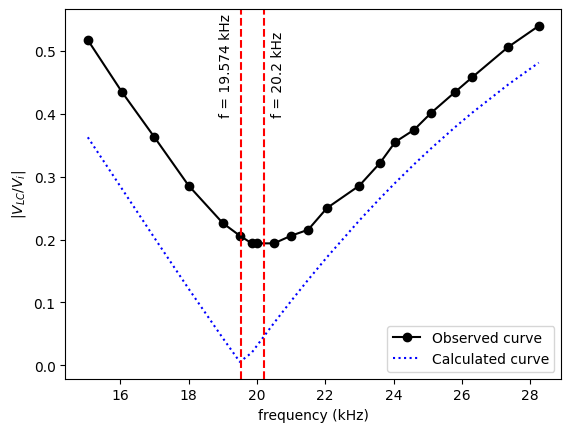
\includegraphics[width=1\columnwidth]{images/g4.png}
            \caption{Observed and computed values of $V_{LC}/V_i$ plotted against input frequency ($R=R_1$)}
            \label{graph:3}
        \end{figure}

        At resonance, $|V_{LC}/V_i|$ should be minimum (ideally 0). From the observed values as shown in Fig. \ref{graph:3}, we can estimate the resonance frequency to be $f_o=20.2$ kHz.

        \begin{figure}[H]
            \centering
            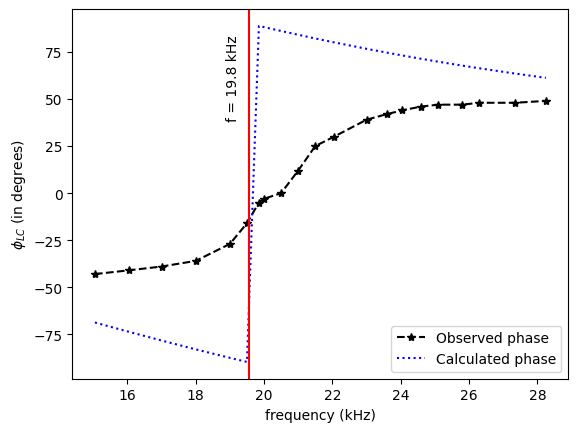
\includegraphics[width=1\columnwidth]{images/g5.png}
            \caption{Observed and computed values of $\phi_{LC}/V_i$ plotted against input frequency ($R=R_1$)}
            \label{graph:4}
        \end{figure}

        At resonance, $\phi_{LC} = 90^{\circ}$, ie. the slope of $\phi_{LC}$ vs $f$ curve changes drastically. Hence from Fig. \ref{graph:4}, we can estimate the resonance frequency to be $f_o=19.8$ kHz.

    \subsection{$V_C/V_i$ and $V_L/V_i$ vs frequency plots}

        \begin{figure}[H]
            \centering
            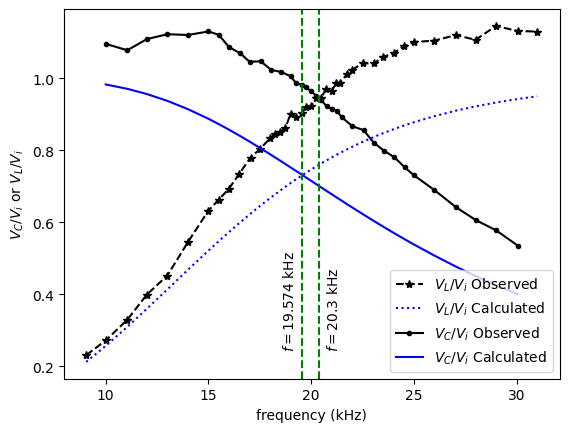
\includegraphics[width=1\columnwidth]{images/g3.png}
            \caption{Observed and computed values of $V_L/V_i$ and $V_L/V_i$ plotted against input frequency ($R=R_1$)}
            \label{graph:5}
        \end{figure}

        At resonance, $V_L = V_C$. Hence, the point of intersection if the two curves in Fig. \ref{graph:5} indicates resonance. For the observed values, the corresponding resonance frequency comes out to be $f_o=20.30$ kHz.
